%
%

% -----------
% 1. Präambel
% -----------

% Allgemeine Einstellungen
% ------------------------
\documentclass[
    pdftex,
	a4paper,
	oneside,
	12pt,
	liststotocnumbered
]{article}

% Meta Information festlegen
\PassOptionsToPackage{hyphens}{url}\usepackage[
	pdftitle={Benefits of Augmented Reality in Educational Environments},
	pdfsubject={},
	pdfauthor={Phil Diegmann, Sven van den Eynden, Manuel Schmidt-Kraeplin},
	pdfkeywords={Augmented Reality, Education, AR, Benefits, Educational},
	colorlinks=false,
	breaklinks=true
]{hyperref}

\usepackage{times}            % Times New Roman
\usepackage{newclude}
\usepackage[ampersand]{easylist}

\usepackage{tabularx}
\usepackage{footnote}
\usepackage{csquotes}
\usepackage[utf8]{inputenc}   % utf-8
\usepackage[T1]{fontenc}      % Umlauttrennung
\usepackage[english]{babel}    % englische Silbentrennung
\selectlanguage{english}       % englische Betitelung
\usepackage{nicefrac}

% Titel-Font-Größen
\usepackage{titlesec}
\titleformat{\section}{\bfseries}{\thesection.}{12pt}{}
\titleformat{\subsection}{\bfseries}{\thesubsection }{12pt}{}

% Seitenränder
\usepackage[
    top=2.5cm, 
    bottom=2.5cm, 
    left=5cm, 
    right=1cm
]{geometry} 

% Fussnoten
% multiple
\usepackage[hang,flushmargin]{footmisc}    
\renewcommand*{\footnotelayout}{\footnotesize} % size of text
\renewcommand{\footnotemargin}{2.2em}          % margin between text and number
\setlength{\footnotesep}{1.3em}                % space between footnotes
\setlength{\skip\footins}{2.5em}               % space between text & footnotes
\usepackage{savefnmark}

\newlength{\arrayrulewidthOriginal}
\newcommand{\Cline}[2]{%
  \noalign{\global\setlength{\arrayrulewidthOriginal}{\arrayrulewidth}}%
  \noalign{\global\setlength{\arrayrulewidth}{#1}}\cline{#2}%
  \noalign{\global\setlength{\arrayrulewidth}{\arrayrulewidthOriginal}}}

% Mehrere Fussnoten mit Komma separieren
\let\oldFootnote\footnote
\newcommand\nextToken\relax

\renewcommand\footnote[1]{%
    \oldFootnote{#1}\futurelet\nextToken\isFootnote}

\newcommand\isFootnote{%
    \ifx\footnote\nextToken\textsuperscript{, }\fi}

% Abkürzungen
%[printonlyused]
\usepackage{acronym}
\renewcommand{\bflabel}[1]{{#1\hfill}}

% Kurzwahlen Directions
\newcommand{\app}{application }
\newcommand{\apps}{applications }
\newcommand{\AR}{AR }
\newcommand{\DBL}{Discovery-based Learning }
\newcommand{\OM}{Objects Modelling }
\newcommand{\ARB}{AR Books }
\newcommand{\ST}{Skills Training }
\newcommand{\ARG}{AR Gaming }
% ns = no space
\newcommand{\appns}{application}
\newcommand{\appsns}{applications}
\newcommand{\ARns}{AR}
\newcommand{\DBLns}{Discovery-based Learning}
\newcommand{\OMns}{Objects Modelling}
\newcommand{\ARBns}{AR Books}
\newcommand{\STns}{Skills Training}
\newcommand{\ARGns}{AR Gaming}

% superscript comma and space
\newcommand{\mulcit}{\textsuperscript{, }}

% paragraph with new line
\newcommand{\heading}[1]{\paragraph*{#1}\mbox{}\\}

% Seitennummerierung oben
\usepackage{scrpage2} 
\usepackage[dvipsnames,usenames]{color}
\clearscrheadfoot 
\chead[\pagemark]{\textcolor[gray]{0.5}{\pagemark}} 
\pagestyle{scrheadings}

% TOC, LOF, FIG Styles
\usepackage{needspace}
\usepackage{tocloft, titletoc}  
\setlength{\cftaftertoctitleskip}{0em}
\renewcommand{\cftloftitlefont}{\bfseries}
%\renewcommand{\cftfigfont}{\bfseries}
\renewcommand{\cfttoctitlefont}{\bfseries}
\renewcommand{\cftlottitlefont}{\bfseries}
\titlecontents{section}     % set formatting for \section 
[2.3em]                     % adjust left margin
{\vspace{0.5em}}            % font formatting
{\hspace{-1.8em}.\contentslabel{0.7em}\hspace{1em}} % section label and offset
{\hspace*{-2.3em}}
{\titlerule*[1mm]{.}\contentspage}

\titlecontents{subsection}  % set formatting for \subsection 
[3em]                       % adjust left margin
{\vspace{0.5em}}            % font formatting
{\contentslabel{2.3em}}     % section label and offset
{\hspace*{-2.3em}}
{\titlerule*[1mm]{.}\contentspage}

\titlecontents{subsubsection}  % set formatting for \subsubsection 
[4.2em]                       % adjust left margin
{\vspace{0.5em}}            % font formatting
{\contentslabel{2.3em}}     % section label and offset
{\hspace*{-2.3em}}
{\titlerule*[1mm]{.}\contentspage}

\titlecontents{figure}      % set formatting for \subsection 
[3.4em]                     % adjust left margin
{\vspace{0.5em}}            % font formatting
{:\hspace*{0.9em}\contentslabel{4.5em}}     % section label and offset
{\hspace*{-2.3em}}
{\titlerule*[1mm]{.}\contentspage}

\titlecontents{table}       % set formatting for \subsection 
[3.4em]                     % adjust left margin
{\vspace{0.5em}}            % font formatting
{:\hspace*{0.9em}\contentslabel{4.5em}}     % section label and offset
{\hspace*{-2.3em}}
{\titlerule*[1mm]{.}\contentspage}


% Literaturverzeichnis
\usepackage[
    bibstyle=authortitle,
    citestyle=authoryear,
    isbn=false,
    url=true,
    doi=false,
    maxcitenames=2,
    maxbibnames=30,
    autocite=footnote
]{biblatex}
\addbibresource{literature.bib}
\let\cite\textcite

\usepackage{caption}
\usepackage{chngcntr}

% Tabellenpackete
\usepackage{array}
\usepackage{xcolor}
\usepackage{longtable}
\usepackage{setspace}
\counterwithin{table}{section}
\usepackage{multirow}
\usepackage{longtable}
\usepackage{float}
\restylefloat{table}
\usepackage{enumitem}
\usepackage{changepage}
\usepackage{pdflscape}
\setenumerate{noitemsep,topsep=0pt,parsep=0pt,partopsep=0pt}

% Grafiken anzeigen
\usepackage[pdftex]{graphicx}
\graphicspath{{figures}}
\usepackage{rotating}
\counterwithin{figure}{section}
\usepackage[absolute,overlay]{textpos}

\setlength{\parindent}{0in}
\interfootnotelinepenalty=10000

\begin{document}

%\shorthandoff{"}

% Variables

% Renews
\renewbibmacro*{cite}{%
  %\global\boolfalse{cbx:loccit}%
  \iffieldundef{shorthand}
    {\ifthenelse{\ifciteibid\AND\NOT\iffirstonpage}
       {\usebibmacro{cite:ibid}}
       {\ifthenelse{\ifnameundef{labelname}\OR\iffieldundef{labelyear}}
          {\usebibmacro{cite:label}%
           \setunit{\addspace}}
          {\printnames{labelname}%
           \setunit{\nameyeardelim}}%
        \iffieldundef{labelyear}
          {}
          {\printtext[parens]{\usebibmacro{cite:labelyear+extrayear}}}}}
    {\usebibmacro{cite:shorthand}}}
\renewcommand{\figurename}{}
\renewcommand{\tablename}{}
\renewcommand\thefigure{Fig. \arabic{section}-\arabic{figure}}
\renewcommand\thetable{Tab. \arabic{section}-\arabic{table}}
\newcommand{\todo}[1]{\textbf{\textsc{\textcolor{Red}{TODO: #1}}}}
\newcommand{\note}[1]{\textbf{\textsc{\textcolor{Cyan}{NOTE: #1}}}}
\renewcommand{\contentsname}{Table of Contents}
\renewcommand{\listtablename}{Index of Tables}
\renewcommand{\listfigurename}{Index of Illustrations}
\renewcommand{\arraystretch}{1.5}

\setcounter{secnumdepth}{5}

\pagenumbering{Roman}

% ---------
% Deckblatt
% ---------
\vspace*{1mm}

% Name
\thispagestyle{empty}
Sven van de Eynden, Manuel Schmidt-Kraeplin, Phil Diegmann

\vspace*{32mm}

% 
\begin{center}
\textbf{
    Selected Issues II
\linebreak
    Major Information Systems
}
\end{center}

\vspace*{32mm}

% Titel
\begin{center}
\LARGE 
Benefits of Augmented Reality in Educational Environments
\end{center}

\vspace*{32mm}

% Themensteller
\begin{center}
Dr. Dirk Basten
\end{center}

\vspace*{32mm}

% Köln, ...
\begin{center}
Köln, Juni 2014
\end{center}

% ------------------
% Inhaltsverzeichnis
% ------------------
\tocloftpagestyle{scrheadings}
\tableofcontents
\newpage

% ---------------------
% Abkürzungsverzeichnis
% ---------------------
\section*{Index of Abbreviations}
\addcontentsline{toc}{section}{Index of Abbreviations}
\begin{longtable}{@{}p{.275\textwidth}@{}p{.725\textwidth}@{}}
\end{longtable}

% -------------------
% Tabellenverzeichnis
% -------------------
\listoftables
\addcontentsline{toc}{section}{Index of Tables}
\newpage

% -------------------
% Abbildungsverzeichnis
% -------------------
\listoffigures
\addcontentsline{toc}{section}{Index of Illustrations}
\newpage

\normalsize
\setstretch{1,5}
\pagenumbering{arabic}

% ------
% Inhalt
% ---------
\section{Introduction}
\subsection{Problem Statement}
I cite.\footnote{\cite{Chang.2014}\label{Chang_2014}}\\
And again.\footnote{\cite{Dunser.2012}} Or again the first footnote.\footref{Chang_2014}
\subsection{Objectives}
\section{Augmented Reality in Educational Environments}

\subsection{Definition of "Augmented Reality"}
Although the term 'Augmented Reality' was coined by Tom Caudell, a former Boeing researcher, in 1990, the concept of augmenting the real world with virtual data was initially used by a number of applications in the late 1960s and 1970s. Since the 1990s, AR was used by some large companies in purpose of visualization and training. Nowerdays, the rising power of personal computers and mobile devices enable the concept of AR to be delivered to traditional educational environments such as schools and universities. \autocite [cf.][21]{Johnson.2010} \\
During the last years the term 'Augmented Reality' has been given different meanings by varying researchers. \autocite [cf.][42]{Wu.2013} \cite{Milgram.1994b} defined AR on the basis of the reality-virtuality continuum (\ref{fig:RealityVirtualityContinuum}) as "augmenting natural feedback to the operator with simulated cues". \autocite[283]{Milgram.1994b} The reality-virtuality continuum (\ref{fig:RealityVirtualityContinuum}) allows us to distinguish the concept of AR to related concepts such as Virtual Reality (VR) where "the participant observer is totally immersed in a completely synthetic world" \autocite[283]{Milgram.1994b} or Augmented Virtuality (AV) where "the the primary world being experienced is in fact [...] predominantly 'virtual'"\autocite[4]{Milgram.1994} and augmented with information from the real world. In addition, \cite{Milgram.1994b} mention a more restricted definiton where AR is seen as "form of virtual reality where the participant's head-mounted display is transparent, allowing a clear view of the real world". \autocite[283]{Milgram.1994b} As suggested by educational researchers,\autocite[cf.][42]{Wu.2013} we reject the idea that the concept of AR is limited to any type of technology. Therefore, we broadly define AR referring to \cite{Klopfer.2008} as "a situation in which a real world context is dynamically overlaid with coherent location or context sensitive virtual information"\autocite[205]{Klopfer.2008} and regard it as a concept which is based on and realized by but conzeptualized beyond technology.
\begin{figure}[ptbh]
    \centering
    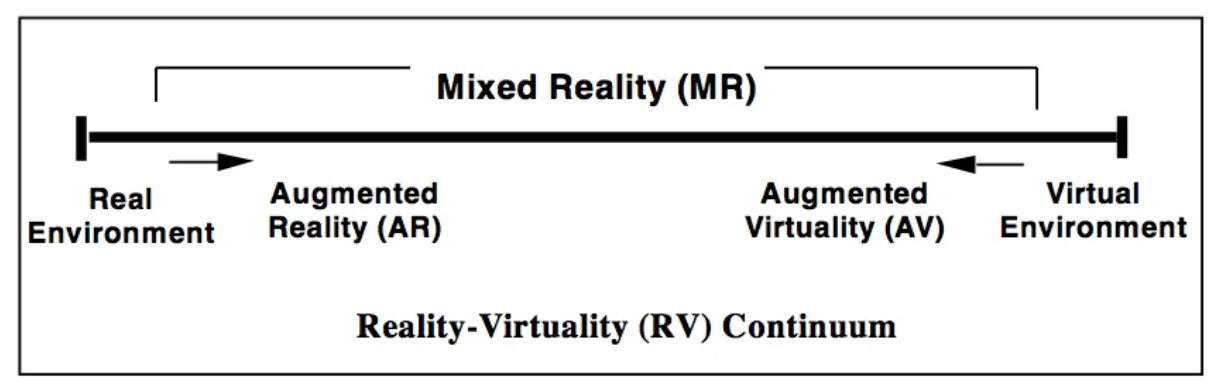
\includegraphics[width=\linewidth]{figures/rvc.png}
    \caption[Reality-Virtuality Continuum]{Reality-Virtuality Continuum}
    \label{fig:RealityVirtualityContinuum}
\end{figure}
\subsection{Five Directions of Augmented Reality in Educational Environments}
\section{Systematic Literature Review}
We applied a two-step research approach, whereby we first conducted a systematic literature review to identify relevant publications before analysing the identified publications for the coding of benefits and directions. After coding, we grouped all found benefits. This process is illustrated in \ref{fig:ResearchApproachGathering} for data collection and in \ref{fig:ResearchApproachAnalysis} for data analysis.

\subsection{Data Collection}
For the identification of papers addressing \AR in educational environments, we applied a systematic online literature database search. We included databases which were specialised on more information systems centered papers, namely Institute of Electrical and Electronic Engineers (IEEE) Xplore Digital Library, ProQuest (ABI / INFORM), Association for Information Systems Electronic Library (AISel) and Association for Computing Machinery (ACM) Digital Library, as well as more general databases, namely EBSCO Host and ScienceDirect.\\
To find relevant papers, we searched within all databases on the following attributes: title, abstract and author supplied keywords. In our query we had three mandatory groups of keywords. Every article had to include the keyword "\AR". Additionally, every article had to have at least one synonym for education and benefits. Namely we searched for "Educat*", "Learn*", "Teach*", "College" or "School" as synonyms for education and "Benefi*", "Advan*", "Improv*", "Enhanc*", "Driver*" or "Value*" as synonyms for benefits. To deal with the limitations of some databases, we had to split our query and conduct multiple queries on the database and merge them together by hand.\\
This database query resulted in a total of 523 articles. Those results were checked against our include- and exclude-criteria, which are listed in \ref{tab:IncludeExcludeCriteria}. We limited the results to empirical works, because we wanted to gain insights into benefits of applied systems and benefits in real-world scenarios. Also, we focused only on positive effects to reduce the amount of data to process. Other aspects we excluded explicitly are non-human learning scenarios like machine learning and learning contexts with special requirements like students with disabilities. Both aspects were left out of our research because they require special attention. \\
This process of data collection was performed by all three authors and each article was read by two of the authors. After merging our results, a total of 25 articles remained.

\begin{figure}[ptbh]
    \centering
    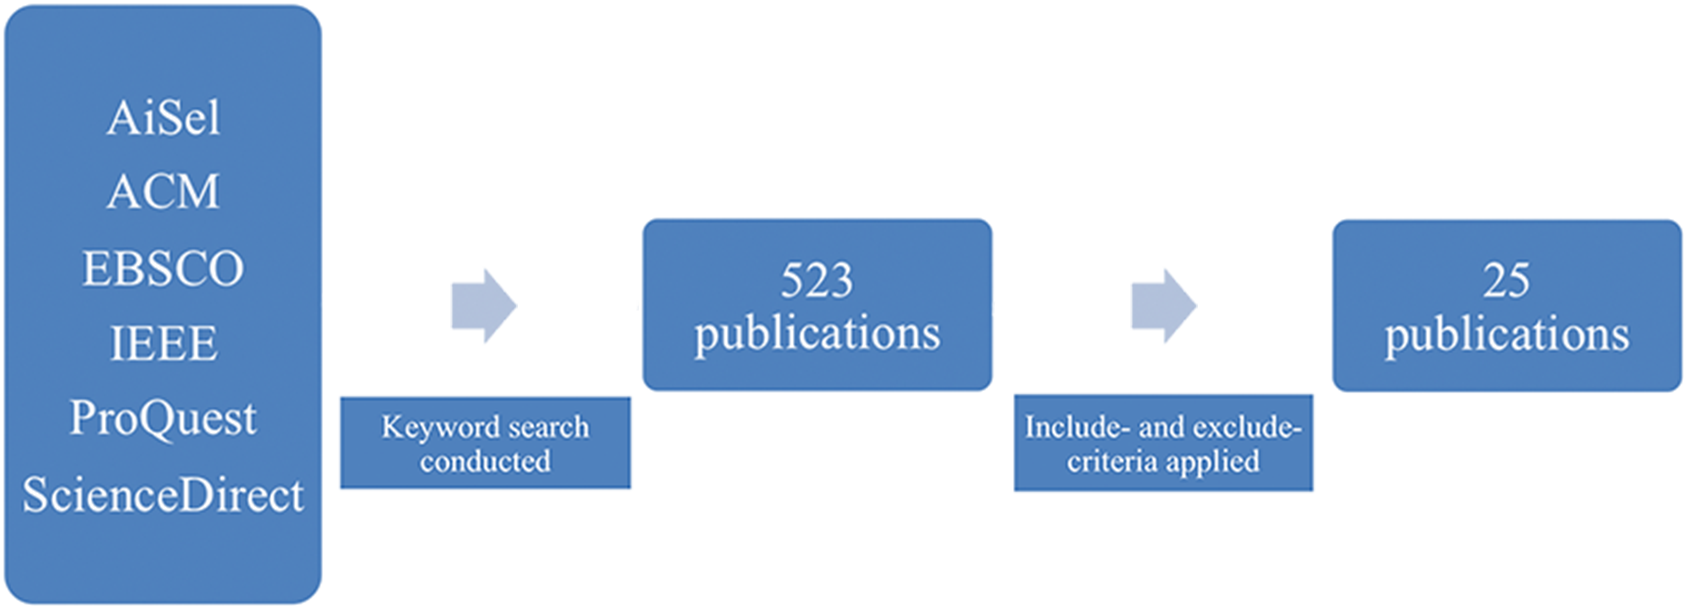
\includegraphics[width=\linewidth]{figures/research_approach_part_1.png}
    \caption[Research Approach: Data Gathering]{Research Approach: Data Gathering}
    \label{fig:ResearchApproachGathering}
\end{figure}

\begin{table}[ptbh]
    \center
    \begin{tabular}{p{16.75em} | p{16.75em}}
        \textbf{Include Criteria} & \textbf{Exclude Criteria} \\
        \hline
        Empirical works & Theoretical works, grey literature, dissertations \\
        A teaching problem is solved with the help of \AR or a teaching concept is improved by \AR & Untried or untested technologies, concepts without empirical evidence \\
        Lists positive effects of \AR applications in comparison to conventional learning tools & No control-group or control-scenario provided, no comparison to conventional learning tools \\
        Human learning & Machine learning \\
        English language & Other language \\
        Peer-reviewed & Not peer-reviewed \\
        Students without disabilities or special requirements & Students with disabilities or special requirements \\
    \end{tabular}
    \caption[Include- and Exclude-Criteria]{Include- and Exclude-Criteria}
    \label{tab:IncludeExcludeCriteria}
\end{table}

\begin{figure}[ptbh]
    \centering
    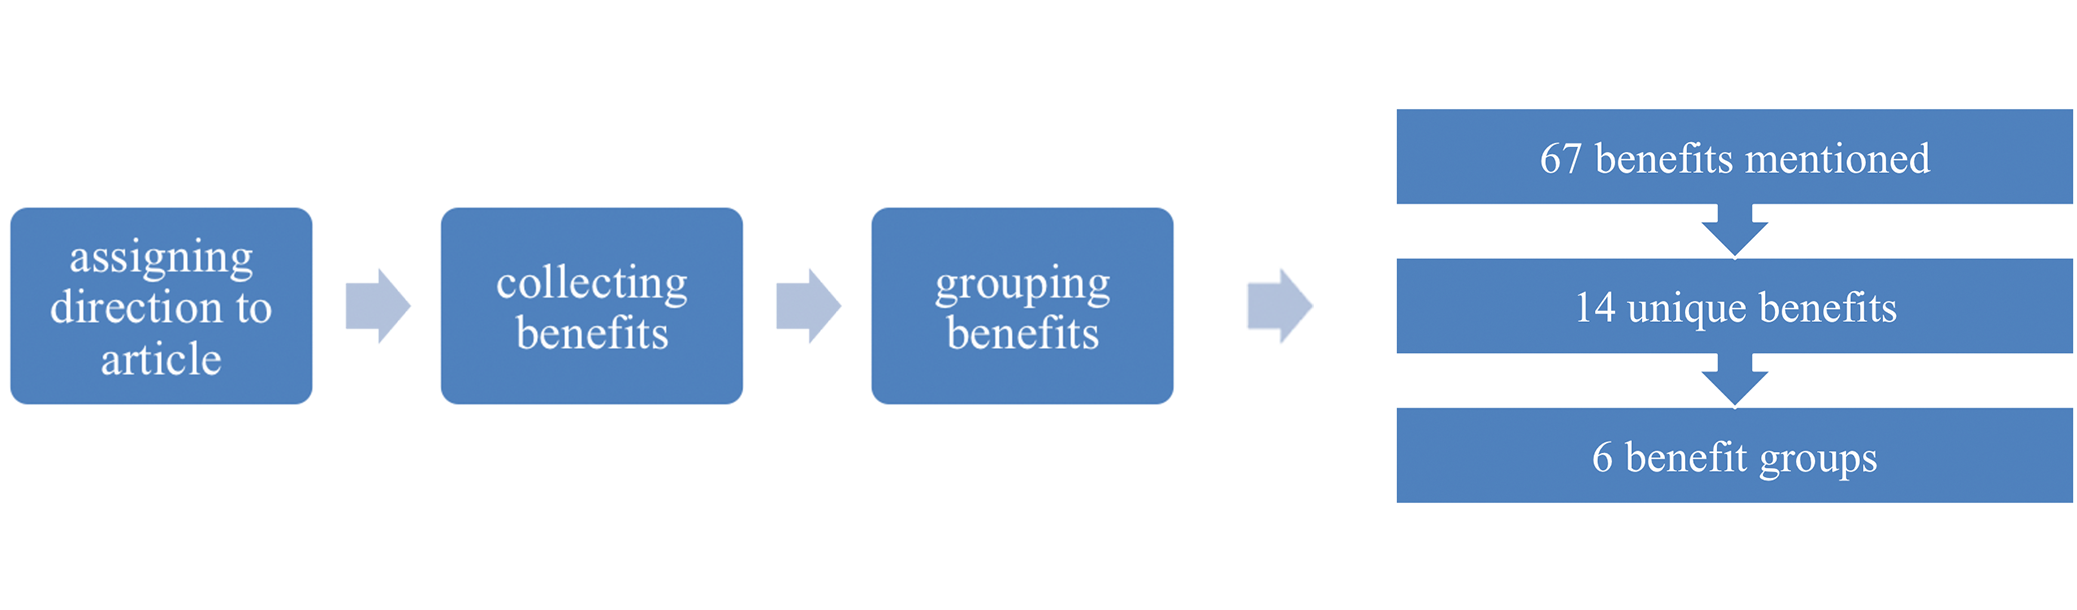
\includegraphics[width=\linewidth]{figures/research_approach_part_2.png}
    \caption[Research Approach: Data Analysis]{Research Approach: Data Analysis}
    \label{fig:ResearchApproachAnalysis}
\end{figure}

\subsection{Data Analysis}
\label{subsec:DataAnalysis}
During data analysis we clustered all found benefits into major groups and matched all found benefits to the directions of the articles in which they were mentioned. We will go into details regarding the benefits found and the clustering of them in chapter \ref{subsec:Benefits} and the mapping process will be highlighted in chapter \ref{subsec:Mapping}.\\
Because of our orientation towards the five directions, we assigned preliminary directions to all articles during data collection but revised our assignment in case of differences between the first and second coder. To measure our precision regarding the coding of the articles into directions, we utilised the inter-coder reliability score, proposed by \cite{Miles.1994}.\autocite[cf.][46]{Miles.1994} This score is calculated by dividing the number of agreements by the total number of agreements and disagreements. Our inter-coder reliability score is 0.64. We will interpret and discuss this score in chapter \ref{sec:Discussion}. \\
During assignment of directions we also collected all mentioned benefits and generalised similar benefits into a single one. Afterwards, those benefits were grouped into broader topic-related benefits. The process we applied is based on the process proposed by \cite{Jankowicz.2004}.\autocite[cf.][149]{Jankowicz.2004} The process proposed by \cite{Jankowicz.2004} helps by formalising the process of clustering.\\
A total of 99 quotes were collected and 67 benefits were mentioned, containing 14 unique benefits, which were clustered into six clusters. In the next chapter, we will introduce all found benefits and their major groups.
\section{Benefits of Augmented Reality in Educational Environments}
\label{sec:Benefits}
In this main-chapter we will present all benefits found. In the first sub-chapter we will present the benefits categorized in five different categories and afterwards we present the mapping of the benefit to the "Five Directions".
\subsection{Benefit Categorization}
\label{subsec:BenefitCategorization}
To improve clarity and to find semantically coherent groups, the benefits were clustered into a category if they are logically related to the same subject, as you can see in the following.

% 
\subsubsection{State of Mind}
In this subsection all benefits are presented which we grouped under the terms 'State of Mind'. These benefits are related to the users state of mind while using the \AR \appns. Some of these benefits can affect 
each other or are intuitive not clearly distinguished such as increased attention and increased concentration. Therefore some quotations could be interpreted as proof for another benefit, as you can see in the following.
However the benefits differ in certain properties which we will point out in the respecting paragraphs. Especially we will pay attention to the benefits 'increased attention' and 'increased concentration' in this respect.
\heading{Increased Motivation}
By increased motivation we mean that users have more eager and interest and are more engaged to deal with the new technology and thus also to deal with the teaching and learning content than by application of non-\AR methods. With a fraction 21,74\% of all benefits mentioned, 
'increased motivation' is after 'improved learning curve' (26.87\%) by far the most mentioned benefit, the third most are 'Reduced Cost' and 'Improved Development of Spacial Abilities' with fractions of 5,8\%.
This is shown by some quotations by \cite{Dunser.2012}, \cite{Iwata.2011}, \cite{Kamarainen.2013}, \cite{Liu.2009b}, \cite{MartinGutierrez.2011}, \cite{MartinGutierrez.2011}, \cite{Tian.2013}, \cite{Redondo.2013}, 
\cite{VateULan.2012} and \cite{Yen.2013}, who present this benefit literally, such as "[...] the AR-style game play successfully enhanced intrinsic motivation towards the self-learning process"\autocite[113]{Iwata.2011}, "Participants 
using the AR books appeared much more eager at the beginning of each session compared with the NAR group"\autocite[112]{Dunser.2012} or "students have been satisfied and motivated by these new methodologies, in all cases"
\autocite[60]{Redondo.2013}. Furthermore it is also shown by some implicit statements like "results showed that students were less bored and more in flow state
when the AR-based application was used during the Magnet\_2 stage"\autocite[8]{Ibanez.2014} or by findings such as the users "were more proactive"\autocite[10]{Chang.2014}\mulcit\autocite[cf.][187]{Zhang.2014} or the will to continue learning using
the AR-Technology after class\autocite[8]{Liu.2009b}. A more detailed description was found also in \cite{Iwata.2011}, where physical interaction is explicit identified as a driver to enhance emotional
engagement.\autocite[cf.][8]{Iwata.2011} Additionally this benefit was found in \cite{Li.2011} and \cite{Hou.2013}.\autocite[cf.][322]{Li.2011}\mulcit\autocite[cf.][448]{Hou.2013}
\heading{Increased Attention}
The benefit 'Increased Attention' is about the amount of attention the user pays to the technology and with this to the teaching and learning content. It is once mentioned literally by \cite{VateULan.2012}.\autocite[cf.][894]{VateULan.2012} In the other two cases, we interpreted the quotations "felt it interesting [...] using the AR-guide system"\autocite[194]{Chen.2008} and 
"teachers noted that the smartphones [the AR-System] promoted interaction with the pond (of which the pupils should learn something about) and classmates"\autocite[552]{Kamarainen.2013} as proof for 
increased attention. As said at the beginning of this chapter, such cases could be interpreted in other ways.
\heading{Increased Concentration}
The difference between the benefits 'increased attention' and 'increased concentration' is just the fact, that we found it literally in the literature. We included it
without any further interpretation or consideration to possible overlapping in the meaning of the terms.
'Increased Concentration' is about the amount of concentration while using \AR \appsns. This benefit was also found for three times. Similar to the detailed description of \cite{Iwata.2011} for increased motivation through \AR \appns, "physical interaction
induced deeper concentration [...]"\autocite[9]{Iwata.2011}, too. \cite{Yen.2013} as well as \cite{Ibanez.2014} perceive an "higher [...] degree of concentration"\autocite[173]{Yen.2013} respectively a 
"higher level of concentration"\autocite[11]{Ibanez.2014}. 
\heading{Increased Satisfaction}
'Increased Satisfaction' means that users experience higher satisfaction regarding the learning process or that users were more satisfied regarding what they have learned after learning with the \AR \app than with the 
conventional method. As an example of more satisfaction regarding the learning process, students have more fun running through a library an solve some tasks directed by an \AR \app than by a librarian\autocite[649]{Chen.2012}.
\cite{MartinGutierrez.2013} says, that "the students were quite satisfied with the [AR-]tools used to learn"\autocite[6]{MartinGutierrez.2013}. A reverse statement therefor is that the frustration level is higher using the 
manual way\autocite[cf.][448]{Hou.2013}. Additionally this benefit is mentioned by \cite{Ibanez.2014} and \cite{Redondo.2013}, so in total five times.

% 
\subsubsection{Teaching Concepts}
During our analysis we observed that two different teaching concepts were supported by AR applications. We clustered these concepts as 'Student Centered Learning' and 'Collaborative Learning' which we explain in the following.
\heading{Increased Student Centered Learning}
Student centered learning is a teaching concept where conventional lectures are replaced by new active and self-paced learning programs. In student centered learning approaches, students are more self-responsible for their own progress in education and educators act as faciliators, who enable the students to learn independently and individualized.\\
Three studies report that AR enabled an increased student centered learning approach in the regarded learning environment. \cite{VateULan.2012} recognizes that the regarded AR application enabled "functionality depended on [...] students’ learning capability" \autocite [894]{VateULan.2012}. Similarly, \cite{Kamarainen.2013} report that "these technologies provide ways of individualizing instruction in a group setting".\autocite[\label{fn:Kamarainen_2013_554}p. 554]{Kamarainen.2013} In addition, \cite{Kamarainen.2013} state that "the technology supported independence" which "freed the teacher to act as a faciliator".\footref{fn:Kamarainen_2013_554} Furthermore, \cite{Liu.2009b} report that AR "improves the ability to explore and absorb new knowledge and solve problems" \autocite[173]{Liu.2009b} which indicates that AR can support student-centered learning environments as students are enabled to explore knowledge and solve problems autonomously. These studies show, that AR can support a student centered learning approach by providing educators with new possibilites to individualize their lessons to students' capability and by enabling students to learn more independently from educators.
\heading{Improved Collaborative Learning}
Three studies report that the regarded AR application improved collaborative learning, meaning that AR enabled new ways of communication and cooperation. \cite{Wang.2012} regard their AR application as "effective environment for conducting collaborative inquiry learning activities". \autocite[57]{Wang.2012} Other authors join the observation of improved collaborative learning as they highlight "the opportunity for collaborative communication and problem-solving among students that arose from the augmented reality experience" \autocite[552]{Kamarainen.2013} and the "facilitation effects of AR technology on collaborative learning effectiveness".\autocite[322]{Li.2011}
% 
\subsubsection{Presentation}
All benefits in the group 'Presentation' are related to the way in which content which should be learned or taught or objects which should support the learning process are visually presented to the user.  
\heading{Increased Details}
The benefit 'Increased Details' is mentioned once. In the context of urban design education the tested \AR "has more detailing particular in the texture of models"\autocite[17]{Chen.2008} than using wood block models of objects for urban 
design learning, as it is the case in the traditional learning method.
\heading{Increased Information Accessibility}
It is reported twice, that \AR \apps improves and eases the access to information regarding the teaching and learning content. In the context of an assembly task guided by an \AR \app instead of an conventional 
assembly manual, \cite{Hou.2013} reports that "[...] AR eases information retrieval by integrating the task of searching information and the task of the actual assembly" \autocite[447]{Hou.2013}. Also \cite{Iwata.2011}
mentions, that "superimposed information was nicely integrated and did not interfere with the learning process"\autocite[112]{Iwata.2011} while learning a traditional Chinese board game.
\heading{Increased Interactivity}
The benefit 'Increased Interactivity' could be seen as a precondition for other benefits presented in this paper, which it is, as you can see in the following and as noted in benefit 'Increased Motivation'. Anyway, increased interactivity through the application of \AR is a 
fact which is not recognised by application of the corresponding conventional method\autocite[cf.][113]{Dunser.2012}\mulcit\autocite[cf.][11]{Ibanez.2014} and therefore specified as a single benefit.
\cite{Dunser.2012} states, that "tangible interaction using tools such as the magnet paddle and augmented nail with labeled poles [in the context of teaching physics] allow for a learning experience that combines real world objects with virtual content. 
Together this can contribute to a deeper understanding. Interactions in AR engage learners with the content, and allow for knowledge to be acquired through their own manipulation of content [...], 
as supported by constructivist learning theory [...]."

% 
\subsubsection{Learning Type}
This subsection deals with benefits we clustered as 'Learning Type'. This group contains benefits which were linked to a specific type of learning, for instance creativity or a more theoretical learning approach like language education. \\
Therefore this group contains two sub-items: improved learning curve and increased creativity. While an improved learning curve is observable on skills based learning, such as spatial skills, or on fields which require a logical understanding, such as languages, increased creativity can be observed on less theoretical grounded areas, such as problem solving or arts.

\heading{Improved Learning Curve}
An improved learning curve, meaning that students learn faster and easier with \AR \apps compared to non-\AR \appsns, is the most often mentioned benefit of \ARns. A total of 26.87\% of all benefits mentioned were related to an improved learning curve. \\
\cite{Liu.2009} reports that "tests taken by the experimental group [the \AR \app users] in all the learning activities were significantly better than those of the control group [the traditionally learning users]".\autocite[525]{Liu.2009} Similarly, \cite{Chang.2014} states, that "[t]he AR-guided group had better learning effectiveness (as evidenced by their posttest scores), and it was found that most visitors believed the AR guide made it easier to digest information than the audio guide due to the extra visual commentary that is provided"\autocite[193]{Chang.2014} as well as "[t]he learning performance of the AR-guided group was thus superior to
that of the other two groups"\autocite[190]{Chang.2014}. More authors join this observation like \cite{Kamarainen.2013} ("[w]e witnessed significant learning gains"\autocite[550]{Kamarainen.2013}), \cite{Ibanez.2014} ("it was found that students who used the AR application performed significantly better on knowledge"\autocite[12]{Ibanez.2014}), \cite{Li.2011}, \cite{MartinGutierrez.2011}, \cite{Redondo.2013}, \cite{Liu.2009b} ("achieved significantly more learning improvement"\autocite[173]{Liu.2009b}), \cite{Zhang.2014}, \cite{Yeo.2011}, \cite{Hou.2013} ("[AR] shortens the learning curve"\autocite[450]{Hou.2013}, "[the] learning curve of trainees significantly improved"\autocite[451]{Hou.2013}), \cite{Wilson.2013} and \cite{Anderson.2013} ("learning [results] increased by more than a factor of 2"\autocite[318]{Anderson.2013}). 
\heading{Increased Creativity}
Increased creativity was mentioned three times (which makes 4,48\% of all reported benefits). For instance, \cite{Liu.2009b} found that "it [AR] also improves student creativity and the ability to explore and absorb new knowledge and solve problems"\autocite[173]{Liu.2009b}. \cite{VateULan.2012} reports, that the "AR 3D pop-up book has highlighted many benefits that include: [...] integration of a variety of learning skills such as [...] and creativity [...]"\autocite[894]{VateULan.2012}. Also, \cite{Chang.2014} observes, that "[o]verall the visitors using the mobile AR-guide system during painting appreciation activities felt that it was an interesting, innovative, creative, and entertaining guide device"\autocite[194]{Chang.2014}. To increase the interpretability of the impact of \AR \apps on creativity, more studies are needed.
% 
\subsubsection{Content Understanding}
The subsection 'Content Understanding' deals with benefits related to the understanding of the learning content by the user and with this the ability to keep the content in memory.
\heading{Improved Development of Spacial Abilities}
The benefit of 'Improved Development of Spacial Abilities' is mentioned four times. \cite{Dunser.2012} for instance says that their "results support the hypothesis, and suggest that Augmented Reality has some potential to be effective 
in aiding the learning of 3D concepts"\autocite[112]{Dunser.2012}. Literally and more detailed, the benefit was found in \cite{MartinGutierrez.2011} as he says that "the training of spatial ability based on 
Graphic Engineering contents and AR technology improves spatial abilities for those who perform them and consequently lower the numbers of students who drop out of the subject"\autocite[5]{MartinGutierrez.2011}.
Additionally this benefit is mentioned by \cite{MartinGutierrez.2013} and \cite{Chen.2008}.\autocite[cf.][4]{MartinGutierrez.2013}\mulcit\autocite[cf.][5]{Chen.2008}
\heading{Improved Memory}
'Improved Memory' refers to the retention of what was learned during the application of the \ARns-method. \cite{Hou.2013} states that "trainees with AR training could remember or recollect more assembly 
clues that were memorized in the former training task than those trained in the manual"\autocite[450]{Hou.2013}. Furthermore it is not only about the mere memory, but also about how vivid the memory is. As \cite{Chang.2014}
says "It [the \AR \app] facilitates the development of art appreciation by imprinting the knowledge of paintings on visitor's memories, supporting the coupling between the visitors, the guide system, and the artwork (Klopfer \& Squire, 2008) by using 
AR technology, and helping visitors keep their memories of the artwork vivid"\autocite[193]{Chang.2014}. Also \cite{Macchiarella.2005} says that \AR "lead[s] to an increased ability to retain long term memories"\autocite[4]{Macchiarella.2005}.
This benefit is mentioned three times in total.

% 
\subsubsection{Reduced Cost}
\cite{Leblanc.2010} and \cite{MartinGutierrez.2011} reported reduced costs in \ARns-scenarios compared to traditional learning in long term. \cite{Chen.2012} highlights especially the low cost in executing manpower and moderate costs for designing and renewing of courses.\autocite[cf.][640]{Chen.2012} \cite{Andujar.2011} join in this point, especially for virtual laboratories.\autocite[cf.][492]{Andujar.2011} \cite{Andujar.2011} add that \ARns-\apps not only reduce direct costs, such as needed materials, but also time for preparing classes. While, at least at the time of this review, \ARns-technology is accompanied with high aquisition cost, this investment will most likely be paid off in the long term. \cite{Leblanc.2010} report, that the one time acquisition cost were high (25.000 US-Dollar)\autocite[253]{Leblanc.2010}, but the cost per class could be lowered by 93,34\% (from 3.000 US-Dollar to 200 US-Dollar)\autocite[253]{Leblanc.2010} which will lead to an overall cost reduction.
\subsection{Mapping of the Benefits to the „Five Directions“}
\label{subsec:Mapping}
Following, we will present the mapping of the found benefits to the five directions. In \ref{tab:MapBenefitsDirections} the mapping results are listed in detail. 

\subsubsection{\DBLns}
We found eight articles (about 32\% of all articles in our result set) whose presented learning concepts were Discovery-based. Those articles had the most mentions of State of Mind benefits, especially increased motivation. 47\% of all increased motivation benefits were related to a Discovery-based \AR application. Also, an improved learning curve was mentioned. About one-third of all improved learning curves were observed in \DBL environments. Nine out of 14 benefits were reported for \DBL applications (about 64\%), which is the most diverse pool of benefits we found during our literature review.

\subsubsection{\OMns}
In our result set of 25 articles, we found five articles, which dealt with an \OM approach for the presented \AR application. Similar to \DBL applications, \OM resulted in an increased motivation and satisfaction. We found about 27\% of all mentions of increased motivation in an \OM context. Also, an improved learning curve was observed. About 22\% of all mentions of an improved learning curve were coherence with an \OM application. It is noticeable, that although \OM itself is highly interactive, we did not find any references of an increased interactivity in classes which used \AR than in classes which did not. None of the \OM applications mention presentation-linked benefits. Also, we found no reports of increased creativity linked to \OM, but spatial abilities were reported to be developed better. Five different benefits were found in \OM applications, which is about 36\% of all reported unique benefits.

\subsubsection{\ARBns}
Two articles (which makes a total of eight percent) were found which were based on an \ARB application. \ARB applications were the least found in the articles. \ARB applications are also connected to an increase in motivation, but not as much as \DBL or \OMns. \ARB seem to provide balanced benefits. Six of 14 benefits were reported in context of \ARB which makes about 43\%.

\subsubsection{\STns}
We found seven articles (about 28 \& of all articles) which presented a \ST \AR application.

\subsubsection{\ARGns}
\ARG was presented in three articles of our result set which accounts for 12 \%. 

\begin{landscape}
\begin{table}[!htb]
    \center
    \begin{adjustwidth}{-1.25cm}{}
    \vspace{-4.45cm}
    \begin{tabular}{c c || c | c | c | c | c || c}
        \textbf{} & \textbf{} & \textbf{\DBLns} & \textbf{\OMns} & \textbf{\ARBns} & \textbf{\STns} & \textbf{\ARGns} & Sums \\
        %\hline
        \Cline{1.0pt}{1-8}
        \textbf{State of Mind} & Increased Motivation & 7 & 4 & 2 & 1 & 1 & 15 \\
        \cline{2-8}
        & Increased Attention & 2 & 0 & 1 & 0 & 0 & 3 \\
        \cline{2-8}
        & Increased Concentration & 2 & 0 & 0 & 0 & 1 & 3 \\
        \cline{2-8}
        & Increased Satisfaction & 1 & 2 & 0 & 1 & 1 & 5 \\
         \cline{2-8}
         & Sums & 12 & 6 & 3 & 2 & 3 & \\
        \Cline{1.0pt}{1-8}
        \textbf{Teaching} & Student Centered & 2 & 0 & 1 & 0 & 0 & 3 \\ \textbf{Concepts} & Learning & & & & & \\
        \cline{2-8}
        & Improved Collective & 1 & 2 & 0 & 0 & 0 & 3 \\ & Learning & & & & & \\
         \cline{2-8}
         & Sums & 3 & 2 & 1 & 0 & 0 & \\
        \Cline{1.0pt}{1-8}
        \textbf{Presentation} & Increased Details & 0 & 0 & 0 & 1 & 0 & 1 \\
        \cline{2-8}
        & Easy Accessible & 0 & 0 & 0 & 1 & 1 & 2 \\ & Information & & & & & \\
        \cline{2-8}
        & Interactivity & 1 & 0 & 1 & 0 & 0 & 2 \\
         \cline{2-8}
         & Sums & 1 & 0 & 1 & 2 & 1 & \\
        \Cline{1.0pt}{1-8}
        \textbf{Learning} & Improved Learning & 6 & 4 & 1 & 6 & 1 & 18 \\ \textbf{Types} & Curve & & & & & \\
        \cline{2-8}
        & Increased Creativity & 2 & 0 & 1 & 0 & 0 & 3 \\
         \cline{2-8}
         & Sums & 8 & 4 & 2 & 6 & 1 & \\
        \Cline{1.0pt}{1-8}
        \textbf{Reduced Costs} & Reduced Costs & 0 & 1 & 0 & 1 & 0 & 2 \\
        \Cline{1.0pt}{1-8}
        \textbf{Content} & Development of & 0 & 2 & 1 & 1 & 0 & 4 \\ \textbf{Understanding} & Spatial Abilities & & & & & \\
        \cline{2-8}
        & Improved Memory & 1 & 0 & 0 & 2 & 0 & 3 \\
        \cline{2-8}
         & Sums & 1 & 2 & 1 & 3 & 0 & \\
    \end{tabular}
    \end{adjustwidth}
    \caption[Mapping of Benefits and Directions]{Mapping of Benefits and Directions}
    \label{tab:MapBenefitsDirections}
\end{table}
\end{landscape}
\section{Discussion}
\label{sec:Discussion}
%Beginn mit Vergleich zu Radu: Ähnlichkeiten: Spatial abilities, long term memory, collaboration, motivation. Seine Einzelbenefits (Content Understanding, language association, physical task performance) wird bei uns als improved learning curve zusammengefasst und ergibt sich bei uns aus der Art der Applikation und dem benefit learning curve. Z.B. direction "skills training" mit benefit learning curve = improved physical task performance. Den Benefit spatial abilities haben wir hingegen als eigenen Benefit gewählt weil durch den Einsatz von AR ein neues Level von Spatial abilities erreichen können und nicht nur die learning curve improved ist. (Evtl gutes Zitat)
In comparison to \cite{Radu.2014}, our study has some similarities as well as some distinctions. \cite{Radu.2014} mentions "spatial abilities", "long term memory, collaboration" and "motivation". We found these benefits as well and therefor inherited them. But in contrast to \cite{Radu.2014}, we condensed "content understanding", "language association" and "physical task performance" into "improved learning curve". Depending on the direction of the \appns, we are able to disaggregate our condensed "improved learning curve" benefit into a more detailed benefit, i.e. a \ST \app with an improved learning curve is equal to "physical task performance". We have to mention, that we have chosen to define "Development of Spatial Abilities" as another benefit and even in another group, as some \apps lead to a new level of spatial abilities which might not have been achieved without \AR or is at least extraordinary improvements in spatial abilities. \cite{MartinGutierrez.2013} states, that "[...] the students have a probability of over 95\% of improving their levels of spatial ability when performing the proposed training. Besides this, results show there is no improvement in control group levels"\autocite[4]{MartinGutierrez.2013} which indicates that spatial abilities were improved far more than usual. \\
% passt das? "[t]he training of spatial ability based on Graphic Engineering contents and AR technology improves spatial abilities [...] lower[s] the numbers of students who drop out of the subject."\autocite[5]{MartinGutierrez.2011}

A larger difference compared to \cite{Radu.2014} is, that we segmented attention into two subcategories, namely concentration and attention. While \cite{Radu.2014} states that \AR \apps might fail to improve student's attention or lead to an unintended focus on the technology itself and not the topic\autocite[cf.][314]{Radu.2014}, we found articles that state the opposite. \cite{Kamarainen.2013} states, that "[t]he teachers stated that they began this project with skepticism about whether the technology would overwhelm the experience, holding the students’ attention at the expense of their noticing the real environment. However, teachers and investigators found the opposite to be true. Students were captivated when a squirrel dropped a seed from a tree near the path and nearly hit a classmate; they called out excitedly when they observed a frog near the shore."\autocite[554]{Kamarainen.2013}, and therefor we think, that the drawback mentioned by \cite{Radu.2014} might be related to system design. Furthermore our segmentation into attention and concentration is based on the findings by \cite{Kamarainen.2013}. Attention relates to only an increased awareness of the situation and a focus on the broader environment, while concentration refers to an increased awareness of the topic or subject and an high level of cognitive activity.

% Unterschiede: Motivation 
%
% !!! MEINST DU EVTL. CONCETRATION / ATTENTION? !!! 
% 
% haben wir aufgeteilt in 2 Unterkategorien. Hier nochmal begründen warum wir das gemacht haben und dass wir das durchaus für Sinnvoll erachten da Unterscheidungen zu treffen. Attention hat er als Nachteil gecoded. Da also durchaus ein großer Unterschied. Evtl der Hinweis darauf, dass beides der Fall sein kann, aber bei gut designter Applikation eher Vorteil (Gibt ein sehr gutes Zitat mit diesen ponds wo die autoren eine sinkende Attention befürchtet haben aber genau das Gegenteil war der Fall!)

Some benefits we found were not mentioned by \cite{Radu.2014}, namely reduced costs, student-centered learning, creativity as well as all presentation-related benefits, like increased details, easy accessible information and interactivity.\\
% Benefits die wir zusätzlich haben: Reduced Costs, student-centered learning, creativity und alle presentation benefits.

Regarding increased creativity as one benefit of \AR \appsns, we would not have thought of creativity as one benefit in advance. On the contrary, we would have assumed, that a linear learning tool as \AR \appsns, which are only able to display information that someone added by hand and interact in ways which are predefined. Our findings conversely show that a linear learning tool as \AR \apps is able to support creative, non-linear learning. This finding also stresses, that \AR is a very flexible tool, which can be used in many educational environments and settings and for very different purposes - if it is applied thoroughly. % TODO: Neue Lehrformen und so
\\
% Guter Übergang um auf creativity und student-centered learning. Hier nochmal darauf eingehen, dass wir nicht damit gerechnet hätten, dass auch die creativity so gut unterstützt wird. (AR als lineares Tool (Phil hatte da was gutes gesagt? :D). Creativity zeigt, dass AR wirklich ein Tool ist, was in enorm vielen educational Bereichen eingesetzt werden kann. Student-centered learning ist besonders interessant, da gerade der konventionelle Frontunterricht in viele Fällen nicht mehr zeitgemäß ist (Hier wäre ein gutes Zitat wichtig) und durch neue Lehrformen wie das student-centered learning ersetzt wird. AR kann gerade in diesem Bereich helfen diese neuen Lehrformen voran zu bringen und die Lehre zu verbessern.

\DBL seems to be a very promising \AR direction. As outlined in \ref{subsubsec:DiscoveryBasedLearning} it has benefits ranging from increased motivation, improved learning curve to reduced costs and supports student-centered learning, as supporting a \DBLns-approach, the student is the center of the learning process and the learning process is adjusted to the student's needs and preferences. We could imagine this to be the way students learn in future. \\
% Besonders Geeignet scheint hierbei auch der discovery-based learning approach zu sein, der offensichtlich sehr gut von AR unterstütz wird. (Nochmal kurz auf die vielen Benefits eingehen) Evtl auch auf Verbindung discovery-based und student-centered learning eingehen, da discovery-based eine Ausprägung von student-centered sein kann? --> Lernen der Zukunft?
\\
Our study is limited by a number of factors. Firstly, some of the regarded empirical studies are only informal investigations with a low number of participants. The significance of the ascertained benefits of AR applications may be unclear in these cases. In addition, for some of the regarded directions we did not find enough articles in order to make a point about the diversity of benefits in comparison to other directions. However, AR is one of the most emerging technologies in education and the fact that 15 out of 25 articles we regarded were published in 2012 or later shows that these limitations can be overcome in the future when more empirical evaluations of AR applications in educational environments will be published. Once enough articles have been published we would suggest to investigate every direction of AR in education separately with a decent amount of regarded articles in order to find out more about the diversity of benefits between directions. \\

Another factor which limits our study is revealed by the inter-code reliability of 0.64 regarding the classification of articles to a certain direction of AR. We think that this rather low value can be explained by the circumstance that some articles can not precisely be classified to a single direction, e.g. a discovery-based learning application which uses game elements. In addition, the definitions by \cite{Yuen.2011} leave some room for interpretation which we tried to reduce during our systematic literature review.
\\

While \cite{Radu.2014} states also (potential) negative aspects of \AR in educational environments, we focused on benefits, although negative aspects might offset benefits. \\
% Evtl Zusätzlich in limitations: Wir haben nur benefits betrachtet. Diese können natürlich auch von Nachteilen aufgehoben werden. Radu nennt potentielle Nachteile in seinem Paper.

Another aspect we left out are "special learners": while handicapped people have (sometimes) special requirements, we focused on more general aspects of \AR in educational environments. \\
%Evtl Zusätzlich in limitations (oder conclusion): Wir haben keine "Special Learner" betrachtet. Gerade für diese Gruppe ist aber AR besonders interessant! (Evtl. Zitat) 
% 
% Vielleicht diesen Teil eher in der Conclusion, aka future research?
% 
%Erklären warum das notwendig war und dass man diese Gruppen gesondert betrachten sollte, da hier erhebliches Potential für education besteht!

% Siehe Conclusion: Finally, we want to stress, that each \AR \app is in it's own way unique and there for it is not always easy to generalise. Each \app has to be implemented thoroughly to prevent drawbacks in user interaction or system failures in order to profit from benefits.
%Evtl Zusätzlich in limitations (oder Conclusion): Jede AR application ist einzigartig, daher sind benefits nur sehr schwer generalisierbar. Eine Applikation muss auf jeden Fall vernünftig umgesetzt sein (z.B. ausreichendes Maß an usability) um von den potentiellen Vorteilen zu profitieren.
\section{Conclusion}
Each \AR \app is unique regarding its implementation and especially its purpose on how to support which subject. Hence it is difficult to generalize the benefits, even if they are mentioned literally in the articles.
By doing so, there should be paid special attention on how the author uses the terms of the benefit and how he understand them to prevent misunderstandings and bad, unclean results. Further the application has to be a final 
and well implemented version and no kind of test version to derive valid benefits of \AR from its application and empirical test. The usability of the \AR application for instance should be at its maximum to 
benefit from its application and potential benefits. \\
All in all and apart from that, we found 14 different, frequently mentioned benefits of \AR in our source literature out of which two benefits ('Improved Learning Curve' and 'Increased Motivation') account for over 20\% 
of all benefits mentioned. Hence, on these benefits should be a focus in future work assessing \AR \apps in educational environments under consideration of what was noted in the discussion chapter.


%Evtl Zusätzlich in limitations (oder Conclusion): Jede AR application ist einzigartig, daher sind benefits nur sehr schwer generalisierbar. Eine Applikation muss auf jeden Fall vernünftig umgesetzt sein (z.B. ausreichendes Maß an usability) um von den potentiellen Vorteilen zu profitieren.
%(SVEN)------ sollte auf jendefall in limitations finde ich ----->Evtl Zusätzlich in limitations (oder conclusion): Wir haben keine "Special Learner" betrachtet. Gerade für diese Gruppe ist aber AR besonders interessant! (Evtl. Zitat) Erklären warum das notwendig war und dass man diese Gruppen gesondert betrachten sollte, da hier erhebliches Potential für education besteht!

\renewcommand{\arraystretch}{1.0}

% --------------------
% Literaturverzeichnis
% --------------------

\newpage
\patchcmd{\bibsetup}{\interlinepenalty=5000}{\interlinepenalty=10000}{}{}
\printbibliography[title={Bibliography}]
\addcontentsline{toc}{section}{Bibliography}


% ---------
% Anhang
% ---------

\end{document} 